\chapter{Revisão Bibliográfica}
	\chapterprecis{Teste, teste}
	
	\section{Laboratório de Operações e Processos}
		O Laboratório de Operações e Processos (LOP) é um dos diversos laboratórios para fins de ensino e pesquisa pertencentes ao Departamento de Engenharia Química da UFMG (DEQ). Ainda existem outros laboratórios vinculados ao departamento cuja finalidade é prestar serviços às comunidades interna e externa à UFMG \footnote{\url{http://www.deq.ufmg.br/departamento/infraestrutura}}.
		
		O LOP possui quatro plantas didáticas: \textbf{explicar aqui brevemente as 4 plantas constituintes do laboratório}
		
		%explicar aqui agora sobre a planta de trocador existente
		O trocador de calor existente no laboratório, cuja imagem pode ser vista na \autoref{img1}, é do tipo \textcolor{red}{tubular}. 
		
		\begin{figure}[!htb]
			\centering
			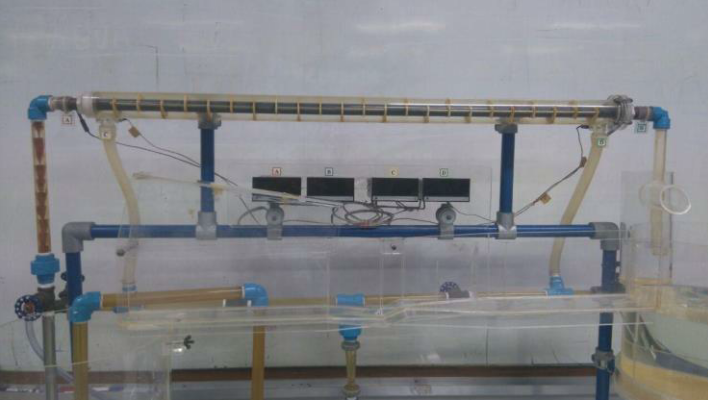
\includegraphics[width=15cm]{img1}  %pode alterar o tamanho
			\caption{Trocador de Calor presente no LOP.}
			\label{img1}
		\end{figure}
	
		Este trocador de calor foi instalado no laboratório em \textcolor{red}{colocar aqui a história do trocador de calor} e originalmente possuía apenas a indicação das medidas de temperatura. A imagem destaca os sensores de temperatura instalados inicialmente. A medição de vazão era inferida através da utilização de uma Calha Parshall\footnote{\url{http://www.dec.ufcg.edu.br/saneamento/PARSHALL.html}}.
			
		Em 2016, um projeto de modernização desta planta foi iniciado por \cite{luiz2016}.  O projeto consistiu na implementação de um sistema embarcado para monitoramento, operação e controle da planta. Para alcançar o objetivo, foram feitos os seguintes passos:
		\begin{itemize}
			\item 
			Instalação de quatro novos sensores de temperatura, dois novos sensores de vazão, tornando possível a medição digital das vazões, 2 relés, para o controle do acionamento dos atuadores e um inversor de frequência para controlar a rotação da bomba;
			\item 
			Instalação de um Arduino Due \footnote{\url{https://store.arduino.cc/usa/arduino-due}} para fazer a interface com sensores e atuadores, processar os algoritmos de controle, e exibir os dados em um display LCD. O programa criado no Arduino possibilita a operação em modo automático e manual;
			\item 
			Construção e instalação de um painel para operar e visualizar os dados da planta. Através desse painel é possível selecionar o modo de funcionamento da planta (manual ou automático). Em modo manual, é possível ligar e desligar bomba e aquecedor, bem como controlar a velocidade da bomba e potência do aquecedor. O display LCD permite exibir várias informações como por exemplo valores das temperaturas e vazões, bem como a sintonia dos controladores. Essas informações não conseguem ser expostas ao mesmo tempo para o usuário, portanto um sistema de navegação foi implementado no Arduino. O esboço do painel elaborado é mostrado na \autoref{img2}.
			
			\begin{figure}[!htb]	
				%\centering
				\captionsetup{justification=centering}
				\begin{center}
					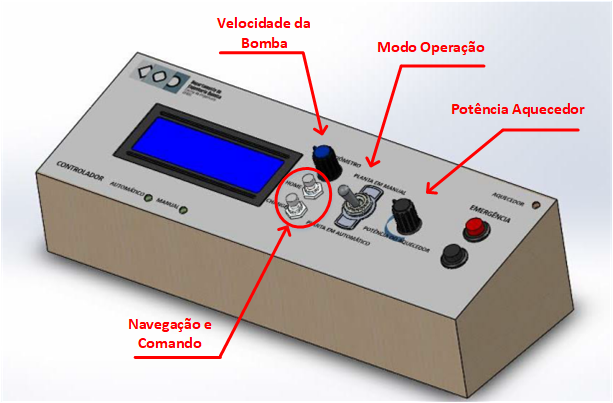
\includegraphics[width=12cm]{img2}  %pode alterar o tamanho
					\caption[Painel instalado na planta de trocador de calor]{\label{img2}Painel instalado na planta de trocador de calor. \\Adaptado de \cite{luiz2016}}
				\end{center}		
			\end{figure}
		
		\end{itemize}
	
	\section{Controle e Monitoramento de Processos Industriais}
		